\chapter{Literature Review}\label{chapter:literature-review}

%==============================================
%      SECTION
%==============================================
\section{Performance Based Standards (PBS)}\label{section:performance-based-standards}
The following section explains the \gls{pbs} framework and highlights the positive impact it has had on the South African economy, society and infrastructure.

%      SUBSECTION
%----------------------------------------------
\subsection{PBS Framework}\label{section:pbs-framework}
  The South African PBS framework is based on the Australian PBS scheme \cite{NationalTransportCommission2008}. It can be broken down into a set of 16 performance measures, 4 infrastructure standards (beyond the scope of this project) and a range of manoeuvres the vehicle is required to perform. 

  The manoeuvres and the performance measures recorded in each manoeuvre are summarised in Table \ref{table:pbs-performance-test-summary}.

%----------------------------------------------
%      TABLE
%----------------------------------------------
  \begin{table}
    \centering\footnotesize
    \caption{PBS manoeuvres and related performance measures}
    % \rowcolors{1}{white}{gray!25}
    \begin{tabulary}{\textwidth}{LL}
      \toprule
        \textbf{PBS Performance Test}	 & \textbf{Performance Measures}\\
      \midrule
        Low speed 90\degree{} turn & LSSP, FS, MoD, DoM, TS, STFD \\
        High speed travel along an unevenly surfaced straight road & TASP \\
        Pulse steer test & YDC \\
        Tilt-table test & SRT \\
        Evasive lane-change procedure (ISO 14791) & RA, HSTO \\
        Acceleration or starting from rest on an upgrade & STA \\
        Maintaining speed on an upgrade & GRAa \\
        Maintaining highest speed on a 1\% upgrade & GRAb \\
        Acceleration from rest to travel 100 m on a flat road & ACC \\
      \bottomrule
    \end{tabulary}%
    \label{table:pbs-performance-test-summary}
  \end{table}%
%----------------------------------------------
%      TABLE
%----------------------------------------------

The vehicle performance is categorised according to the performance Level of the performance measure in which the combination achieved the worst performance. The performance requirements decreases in stringency from Level~1 to Level~4.

\begin{enumerate}
  \item Level 1: General Access
  \item Level 2: Significant Freight Routes
  \item Level 3: Major Freight Routes
  \item Level 4: Remote Areas
\end{enumerate}

The performance measures relevant to this research can be grouped as \gls{ps}, \gls{ss}, \gls{vm}, \gls{rh} and \gls{tdp}~\cite{Arredondo2012}. The performance requirements for each of the measures as adopted by the SMART truck committee in South Africa (as of 1 Jan 2018) for each PBS level are summarised in Table~\ref{table:pbs-performance-measure-requirements}.

%----------------------------------------------
%      TABLE
%----------------------------------------------
  \begin{table}[H]
    \centering\footnotesize
    \begin{threeparttable}
      \caption{PBS performance measures and level requirements}
      \label{table:pbs-performance-measure-requirements}
      \begin{tabular}{crcccccc}
        \toprule
        \multicolumn{4}{r}{}        & \multicolumn{4}{c}{\textbf{PBS Level}} \bigstrut\\ \cline{5-8}
        \textbf{Category} & \multicolumn{1}{c}{\textbf{Performance measure}} & \multicolumn{1}{c}{\textbf{Unit}} & \textbf{Req.} & \textbf{1} & \textbf{2} & \textbf{3} & \textbf{4} \bigstrut\\
        \hline
        \multirow{4}[8]{*}{PS} & \gls{sta} & \%    & $\geq$  & 15    & 12    & 10    & 5 \bigstrut\\
              & \gls{graa} & \%    & $\geq$  & 20    & 15    & 12    & 8 \bigstrut\\
              & \gls{grab} & km/h  & $\geq$  & 80    & 70    & 70    & 60 \bigstrut\\
              & \gls{acc} & s     & $\leq$  & 20    & 23    & 26    & 29 \bigstrut\\
        \hline
        \multirow{2}[4]{*}{SS} & \gls{srt} & g     & $\geq$  & \multicolumn{4}{c}{0.4\tnote{1}, 0.35\tnote{3}} \bigstrut\\
              & \gls{ydc} & -     & $\geq$  & \multicolumn{4}{c}{0.15} \bigstrut\\
        \hline
        \multirow{5}[10]{*}{VM} & \gls{fs} & m     & $\leq$  & \multicolumn{4}{c}{1.5\tnote{1}, 0.7\tnote{3}} \bigstrut\\
              & \gls{dom} & m     & $\leq$  & \multicolumn{4}{c}{0.2} \bigstrut\\
              & \gls{mod} & m     & $\leq$  & \multicolumn{4}{c}{0.4} \bigstrut\\
              & \gls{ts} & m     & $\leq$  & 0     & 0.4   & 0.4   & 0.5 \bigstrut\\
              & \gls{lssp} & m     & $\leq$  & 7     & 8.7   & 11    & 14 \bigstrut\\
        \hline
        RH    & \gls{stfd} & \%    & $\leq$  & \multicolumn{4}{c}{80} \bigstrut\\
        \hline
        \multirow{3}[6]{*}{TDP} & \gls{tasp} & m     & $\leq$  & 3     & 3     & 3.1   & 3.3 \bigstrut\\
              & \gls{ra} & -     & $\leq$  & \multicolumn{4}{c}{5.7$\times$SRT} \bigstrut\\
              & \gls{hsto} & m     & $\leq$  & 1     & 0.8   & 1     & 1.2 \bigstrut\\
        \bottomrule
      \end{tabular}%
    \begin{tablenotes}
      \item[1] Road tankers hauling dangerous goods in bulk, buses and coaches
      \item[2] Buses
      \item[3] Others
    \end{tablenotes}
    \end{threeparttable}
  \end{table}%
%----------------------------------------------
%      TABLE
%----------------------------------------------

%      SUBSECTION
%----------------------------------------------
\subsection{PBS Pilot Project in South Africa and Its Benefits}\label{section:pbs-pilot-project-in-south-africa}

    The PBS framework was adopted in South Africa in 2007. Since its inception, PBS vehicles have been monitored and data from their operation has been recorded. As of June 2017, over 100 million km were travelled by PBS vehicles within the South African road network. Details of the PBS vehicles in operation as part of the pilot project are summarised in Figure~\ref{figure:summary-of-operating-pbs-vehicles-and-commodities-in-south-africa-june-2017}.

%----------------------------------------------
%      FIGURE
%----------------------------------------------
    \begin{figure}[H]
        \centering
        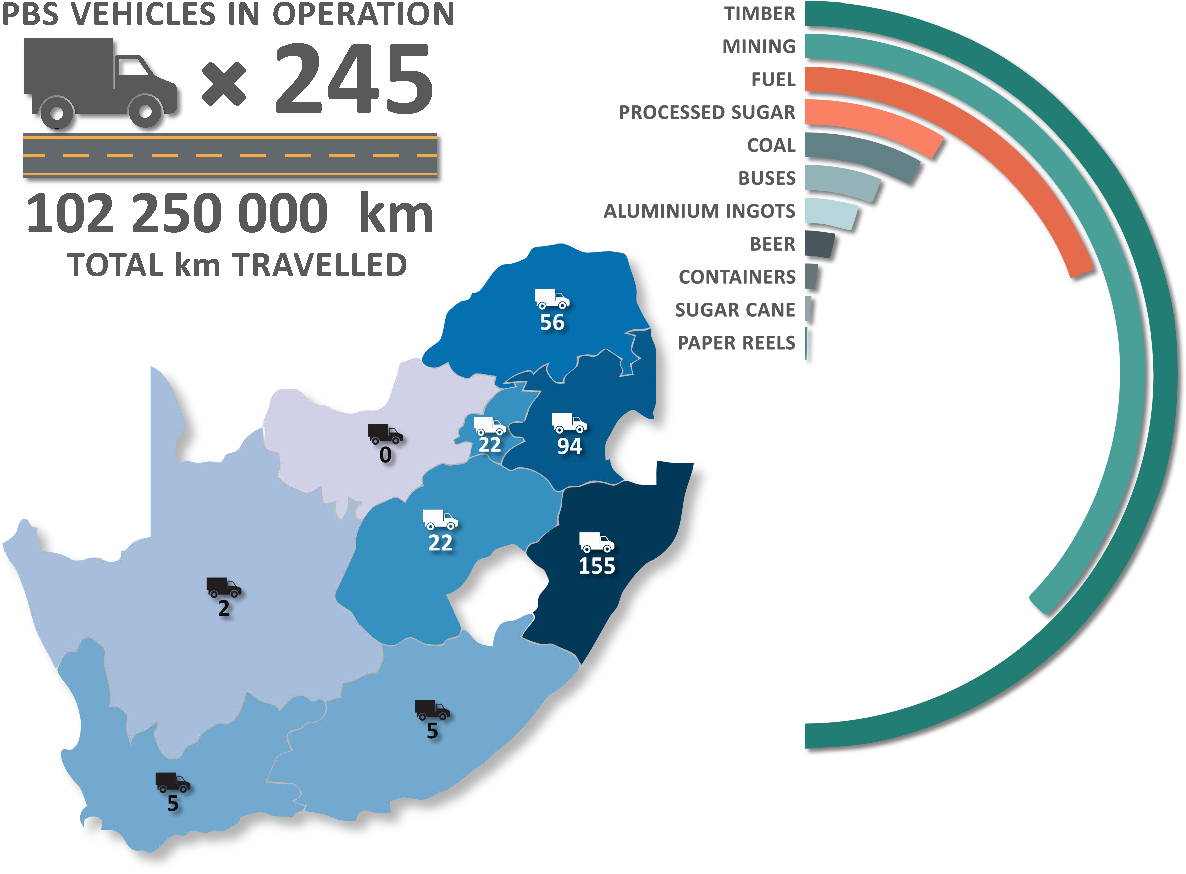
\includegraphics[width=1\textwidth]{fig/pbs-pilot_vehicles-and-commodities-june-2017}
        \caption{Summary of operating PBS vehicles and commodities in South Africa as of June 2017 \cite{Nordengen2018}}
        \label{figure:summary-of-operating-pbs-vehicles-and-commodities-in-south-africa-june-2017}
    \end{figure}
%----------------------------------------------
%      FIGURE
%----------------------------------------------

    The monitoring data that has been collected and analysed for the duration of the PBS pilot project shows PBS vehicles require less trips to transport the same amount of payload which leads to reductions in fuel usage and CO\textsubscript{2} emissions. PBS vehicles are recorded to have a 39\% reduction in accidents relative to their baseline equivalents. This highlights the improved safety performance of the PBS vehicles. The monitoring data shows that the PBS vehicles operating as of June 2017 were saving 74067 trips per year which resulted in R~26.64 million of fuel saved and a reduction of 6246 tons of CO\textsubscript{2}. Each \gls{pbs} vehicle saves R~24448 in road wear per vehicle per year and \gls{pbs} vehicles have a 39\% reduction in accidents relative to their baseline equivalents (see Figure~\ref{figure:summary-of-pbs-monitoring-data-june-2017}).

%----------------------------------------------
%      FIGURE
%----------------------------------------------
    \begin{figure}
        \centering
        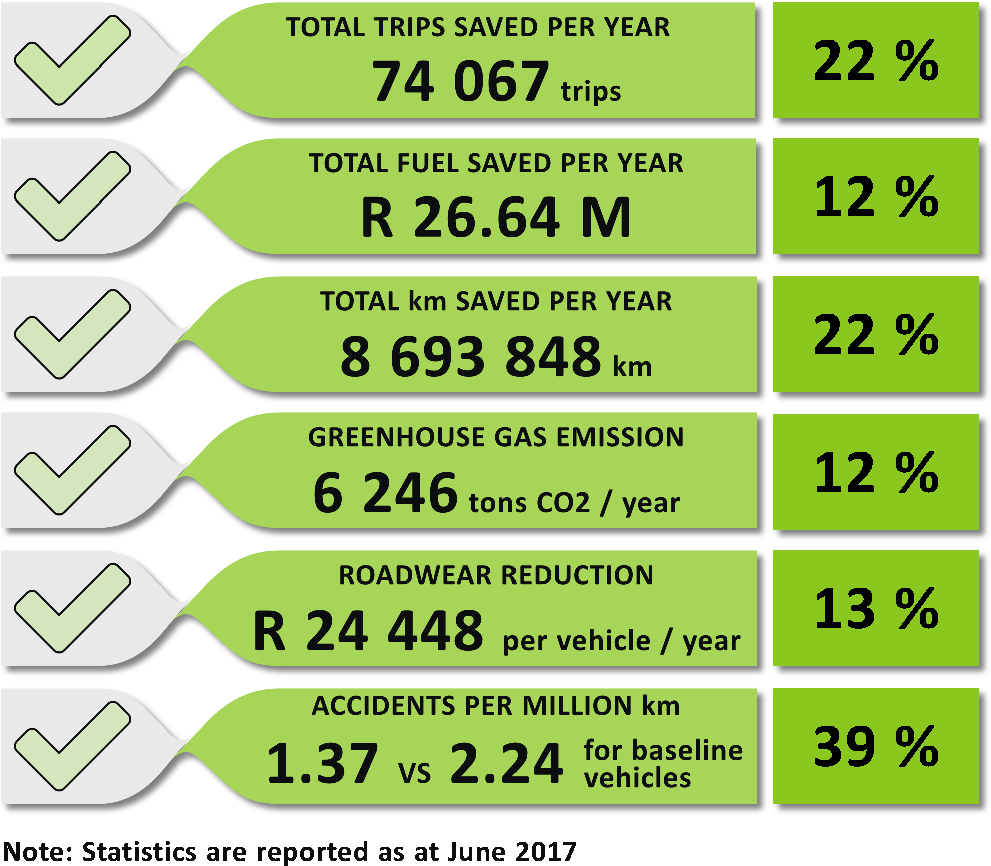
\includegraphics[width=1\textwidth]{fig/pbs-pilot_yearly-statistics-june-2017}
        \caption{Summary of PBS monitoring data as of June 2017 \cite{Nordengen2018}}
        \label{figure:summary-of-pbs-monitoring-data-june-2017}
    \end{figure}
%----------------------------------------------
%      FIGURE
%----------------------------------------------

  The benefits realised by the small sample of \gls{pbs} vehicles is clear. Increasing participation in the \gls{pbs} project will improve the productivity of the South African logistics, decrease the environmental impact of transport operations and reduce damage to infrastructure. Thus, it is beneficial to make the \gls{pbs} assessment process as attractive and efficient as possible to motivate more parties to participate.

%==============================================
%      SECTION
%==============================================
\section{Towards Quicker PBS Assessments}\label{section:towards-quicker-pbs-assessments}

The process of performing a \gls{pbs} assessment requires accurate vehicle details to be sourced from \glspl{oem}, the expertise to interpret the information and tools to perform the assessment. The multi-body vehicle dynamics packages required to simulate vehicle performance are expensive, require know-how to correctly build a representative vehicle model and require a significant amount of computational power to operate. 

This leads to a lengthy and computationally expensive process that requires input from multiple experts. Studies that have been done to simplify and speed up the assessment process are explored in this section.

%      SUBSECTION
%----------------------------------------------
\subsection{Pro-forma Design}\label{section:pro-forma-design}

  De Pont~\cite{Pont2010} initially introduced the concept of pro-forma designs to alleviate time and cost constraints of a PBS assessment. The pro-forma design methodology sets geometrical constraints for a vehicle combination. Following these constraints ensures Level 1 PBS conformity for low-speed directional \gls{pbs} performance measures (\gls{fs}, \gls{ts}, \gls{lssp}). The geometrical constraints are generated by means of a parametric sensitivity analysis aimed to investigate the effects of each of the \glspl{hcv} geometrical properties on the low-speed \gls{pbs} performance measures.
  
  A \gls{lsmm} developed by de~Saxe~\cite{Benade2015} was shown to correlate well with \trucksim{} for the car carrier being analysed. The LSMM was therefore used to assess the vehicle performance measures for all assessments and optimisation iterations.

  \matlab{} code was implemented to generate 10 000 vehicle configurations satisfying the generated constraints. The configurations were tested using the LSMM and it was found that each combination satisfied Level 1 PBS performance requirements.

  The pro-forma approach was found to be an effective manner to reduce the cost of PBS assessments by an estimated 1.2~million rand \cite{Benade2015}. However, in its current form, it only ensures compliance with Level~1 low-speed PBS performance measures and further work would need to be performed to ensure complete compliance.

  A similar pro-forma approach has also been developed by the \gls{nhvr} who made blueprint designs for a variety of truck configurations publicly available on their website~\cite{NationalHeavyVehicleRegulator}. Blueprint \gls{hcv} configurations have been pre-approved by the NHVR and designs based on these configurations will shorten the lead time in the PBS approval process.

  %      SUBSECTION
  %----------------------------------------------
\subsection{Predicting PBS Performance}\label{section:optimisation-of-vehicles-within-the-pbs-framework}

Dessein~\cite{Dessein2012} explored consideration of the PBS framework prior to the detail design phase through optimisation of \gls{hcv} design within the \gls{pbs} framework. Simplified models for eight performance measures (\gls{srt}, \gls{ra}, \gls{lssp}, \gls{fs}, \gls{ts}, \gls{sta}, \gls{graa}) were used to estimate the \gls{hcv} performance. Limiting the number of performance measures evaluated allowed the calculations to be automated by using a sequential quadratic programming algorithm within MATLAB.

The routine varied the five vehicle parameters listed for four types of vehicle (A-Double, B-Double, truck and pig trailer, truck and dog trailer):

\begin{itemize}
    \item Number of axles in each axle group
    \item Wheelbases of all vehicle units
    \item Hitch offset
    \item Payload (size/location/density)
\end{itemize}

The optimisation routine considered a Level~2 PBS requirement, and the vehicle configuration yielding the highest payload (and hence highest productivity) was chosen as optimal. The optimised vehicles were compared to those designed using prescriptive methods.

It was discovered that the vehicles designed using a prescriptive approach were in fact more productive than the PBS equivalent for payloads with a density lower than 400 kg/m\ssth{}. This suggests that an optimisation approach would be very useful in evaluating whether a vehicle can be designed to be more productive using the PBS approach; potentially preventing a costly, unsuccessful, iterative design process.

Dessein showed that the prescriptive vehicles failed to meet the PBS Level~2 \gls{srt} requirement of 0.35~g for most payload densities. Dessein highlighted one of the major disadvantages of the prescriptive approach in that it does not directly consider the vehicles safety performance but imposes only geometrical and mass constraints. Importantly, there is an opportunity using the PBS approach to increase safety and reduce road fatalities even if at the lower payload densities there is little scope to increase the vehicle productivity.

The results of the \gls{adr} developed by Dessein indicate that there is a potential for determining an estimated productivity gain of a PBS assessment before detailed design begins. It can also yield optimal \gls{hcv} configurations that can be used as a starting point in the detailed design of the \gls{hcv}, speeding the process up and increasing the probability of PBS approval.

%      SUBSECTION
%----------------------------------------------
\subsection{Machine Learning Models}\label{section:machine-learning models}

Berman et al. \cite{Berman2015} developed a lightweight tool requiring only vehicle geometry to predict the low-speed \gls{pbs} performance measures of a B-double combination. In total 22 input parameters were randomly selected to conduct 10 000 simulations on a B-double. Supervised machine learning techniques were used to develop a model to predict \gls{lssp}, \gls{fs}, \gls{mod}, \gls{dom} and \gls{ts} performance measures from the simulated data. The model provides an accessible way for \glspl{oem} to quickly and accurately evaluate the low-speed PBS performance of their vehicle before a formal PBS assessment without the need for extensive mechanical knowledge of multi-body vehicle dynamics systems using only geometric parameters of the vehicle combination.

Following his initial research, Berman et al. \cite{Berman2016} developed a lightweight prediction tool using neural networks to predict the high-speed performance of a 9-axle B-double combination. Upper and lower bounds were selected for 30 unique input parameters defining the vehicle geometry, payload and suspension. 36 470 vehicle configurations were created using random sampling within the range of each input parameter assuming a uniform distribution. The model can rapidly predict the \gls{hsto}, \gls{srt}, \gls{tasp}, \gls{ra} and \gls{ydc} PBS performance of a 9-axle B-double combination as well as overall \gls{pbs} performance with a high level of accuracy. The model is intended for determining preliminary PBS performance of a vehicle combination as a guide for \glspl{oem} and transport regulators as a precursor to a formal PBS assessment.

%==============================================
%      SECTION
%==============================================
\section{Design Parameter Effect on Vehicle Performance}\label{section:design-parameter-effect-on-vehicle-performance}
The following Section discusses previous studies that have focused on determining the influence of \gls{hcv} design parameters on heavy vehicle safety.

%      SUBSECTION
%----------------------------------------------
\subsection{Influence of Heavy Vehicle Design Parameters on Vehicle Performance}\label{section:australian-study-on-the-influence-of-heavy-vehicle-design-parameters}

Prem et al. \cite{Prem2002} conducted a study on the Australian heavy vehicle fleet to determine the influence of various design parameters on vehicle safety as assessed using the PBS framework. A baseline configuration was chosen for a variety of vehicle configurations. The design parameters were then varied by +/-20\% and the effects on each performance measure were tabulated, indicating the influence of each performance measure using a scale with 4 discrete quantifiers (++, + for improved performance and - -, - for degraded performance). The results of this study are summarised in Table \ref{table:influence-of-design-features-performance-characteristics-of-australian-fleet}.

%----------------------------------------------
%      TABLE
%----------------------------------------------
\begin{table}[H]
    \centering\scriptsize
    \begin{threeparttable}
        \caption{Influence of design features and broad summary of parametric effects \cite{Prem2002}}
        \begin{tabulary}{\textwidth}{|L|c|c|c|c|c|c|c|c|c|c|c|c|c|c|c|}
        \toprule
            \multicolumn{1}{l}{\textbf{Performance measure}} & \multicolumn{1}{l}{\begin{sideways}\textbf{Increase Engine Power/Torque}\end{sideways}} & \multicolumn{1}{l}{\begin{sideways}\textbf{Increase Driveline Gear Ratio}\end{sideways}} & \multicolumn{1}{l}{\begin{sideways}\textbf{Increase CG Height}\end{sideways}} & \multicolumn{1}{l}{\begin{sideways}\textbf{Increase Axle Loads}\end{sideways}} & \multicolumn{1}{l}{\begin{sideways}\textbf{Longer Prime Mover Wheelbase}\end{sideways}} & \multicolumn{1}{l}{\begin{sideways}\textbf{Longer Trailer Wheelbase}\end{sideways}} & \multicolumn{1}{l}{\begin{sideways}\textbf{Longer Dolly Wheelbase}\end{sideways}} & \multicolumn{1}{l}{\begin{sideways}\textbf{Increase Number of Articulation Points}\end{sideways}} & \multicolumn{1}{l}{\begin{sideways}\textbf{Increase Axle Group Spread}\end{sideways}} & \multicolumn{1}{l}{\begin{sideways}\textbf{Increase Coupling Rear Overhang}\end{sideways}} & \multicolumn{1}{l}{\begin{sideways}\textbf{Increase Suspension Roll Stiffness}\end{sideways}} & \multicolumn{1}{l}{\begin{sideways}\textbf{Increase Tyre Cornering Stiffness}\end{sideways}} & \multicolumn{1}{l}{\begin{sideways}\textbf{Increase Front Overhang}\end{sideways}} & \multicolumn{1}{l}{\begin{sideways}\textbf{Increase Rear Overhang}\end{sideways}} & \multicolumn{1}{l}{\begin{sideways}\textbf{Decrease Speed}\end{sideways}} \bigstrut\\
            \hline
            Startability &       & ++    &       & - -    &       &       &       &       &       &       &       &       &       &       &  \bigstrut\\
            \hline
            Gradeability A & ++    & ++    &       & - -    &       &       &       &       &       &       &       &       &       &       &  \bigstrut\\
            \hline
            Gradeability B & ++    & +/-   &       & -     &       &       &       &       &       &       &       &       &       &       &  \bigstrut\\
            \hline
            Acceleration Capability & +     & -     &       & -     &       &       &       &       &       &       &       &       &       &       & + \bigstrut\\
            \hline
            Tracking Ability on a Straight Path &       &       & - -    & - -    & -     & -     & -     & -     & +     & -     & +     & ++    &       &       & ++ \bigstrut\\
            \hline
            Low-speed Offtracking &       &       &       &       & - -    & - -    & -     & ++    &       & +     &       &       & -     &       &  \bigstrut\\
            \hline
            Frontal Swing &       &       &       &       & - -    &       &       &       &       &       &       &       & - -    &       &  \bigstrut\\
            \hline
            Tail Swing &       &       &       &       &       & +     &       &       &       &       &       &       &       & - -    &  \bigstrut\\
            \hline
            Steer Tyre Friction Demand &       &       &       &       & ++    &       &       &       & - -    &       &       &       &       &       &  \bigstrut\\
            \hline
            Static Rollover Threshold &       &       & - -    & -     &       &       &       &       &       &       & +     &       &       &       &  \bigstrut\\
            \hline
            Rearward Amplification &       &       & -     & -     & +     & ++    & +     & - -    & +     & -     & +     & ++    &       &       & ++ \bigstrut\\
            \hline
            High-speed Transient Offtracking &       &       & - -    & - -    & +     & ++    &       &       & +     & -     &       & ++    &       &       & ++ \bigstrut\\
            \hline
            Yaw Damping Coefficient &       &       & - -    &       &       & ++    &       &       & +     &       &       & ++    &       &       & ++ \bigstrut\\
            \hline
            GM per SAR &       &       &       & -     &       &       &       &       &       &       &       &       &       &       &  \bigstrut\\
            \hline
            Horizontal Tyre Forces & - -    &       &       & - -    &       &       &       &       & - -    &       &       &       &       &       &  \bigstrut\\
            \hline
            Max. Effect Relative to Ref. Vehicles &       &       &       & - -    & ++    & ++    & +     &       & +     &       &       &       &       &       &  \bigstrut\\
            \hline
        \end{tabulary}%
        \label{table:influence-of-design-features-performance-characteristics-of-australian-fleet}
        %Enter table label for referencing here
        \begin{tablenotes}
            \item[1] ++ Significant positive effect on performance
            \item[2] + Moderate positive effect
            \item[3] \textit{blank} Little or no influence
            \item[4] - Moderate negative effect
            \item[5] - - Significant negative effect
        \end{tablenotes}
    \end{threeparttable}
\end{table}%
%----------------------------------------------
%      TABLE
%----------------------------------------------

The results of the study conducted by Prem et al. provide useful insight into how the design parameters effect each performance measure within a range of 20\% of the baseline design parameters. The design parameters of a heavy vehicle are often constrained due to manufacturing limitations and regulations that need to be adhered to. A design parameter could heavily influence the performance of a heavy vehicle; however, it may not be possible to alter that parameter due to design and legal constraints. On the other hand, a parameter may have little effect on the vehicle safety performance but be able to be varied within a large range. The study considered a wide range of vehicle configurations and lumped the results of each vehicle into one summarised result. This loses any insights into how the effect of changing certain design parameters may differ between the vehicle configurations.

%      SUBSECTION
%----------------------------------------------
\subsection{The UMTRI Component Factbook}\label{section:umtri-component-factbook}

Fancher et al. at \gls{umtri} compiled a comprehensive document in 1986 detailing the mechanical properties of components used in heavy vehicles, their influences on manoeuvring performance and a collection of parametric data from the United States heavy vehicle fleet \cite{Fancher1986}. The mechanical properties discussed were categorised as follows:

\begin{enumerate}
    \item Geometric layout
    \item Mass distribution
    \item Tyres
    \item Suspensions
    \item Steering systems
    \item Brakes
    \item Frames
    \item Hitches
\end{enumerate}

In each category, the effect of the mechanical properties on vehicle performance was discussed. A summary of the effect of each mechanical property considered is included in Tables \ref{table:effect-of-the-mechanical-properties-of-tyres-on-vehicle-dynamic-performance} to \ref{table:effect-of-the-mechanical-properties-of-mass-distribution-on-vehicle-dynamic-performance}. Steering systems, frames and braking are beyond the scope of this dissertation, however their effects on vehicle dynamic performance are included for completeness and the interest of the reader.

%----------------------------------------------
%      TABLE
%----------------------------------------------
\begin{table}[H]
	\centering\footnotesize
	\begin{threeparttable}
	
        \begin{tabulary}{\textwidth}{lcccccccccc}
            \toprule
            \textbf{Pertinent Mechanical Property} & \begin{sideways}\textbf{Low-speed tracking}\end{sideways} & \begin{sideways}\textbf{Hi-speed tracking}\end{sideways} & \begin{sideways}\textbf{Roll stability}\end{sideways} & \begin{sideways}\textbf{Handling stability}\end{sideways} & \begin{sideways}\textbf{Response time}\end{sideways} & \begin{sideways}\textbf{Rearward amplification}\end{sideways} & \begin{sideways}\textbf{Braking efficiency}\end{sideways} & \begin{sideways}\textbf{Transient braking \& turning}\end{sideways} & \begin{sideways}\textbf{Downhill braking}\end{sideways} & \begin{sideways}\textbf{Response to disturbances}\end{sideways} \\\midrule
            Cornering coefficient $C_{alpha}/F_z$ & -     & Hi    & -     & Hi    & Hi    & Hi    & -     & Hi    & -     & Hi \\
            Curvature in $C_{alpha}$ ($C_{alpha}$ vs Vertical Load) & Low   & -     & -     & Hi    & Low   & Low   & -     & -     & -     & - \\
            Aligning stiffness (pneumatic trail) & -     & -     & -     & Low   & -     & -     & -     & -     & -     & - \\
            Vertical stiffness & -     & -     & Med   & -     & -     & -     & -     & -     & -     & - \\
            Peak friction, $m_p$ & -     & -     & -     & -     & -     & -     & Hi    & Hi    & -     & - \\
            Sliding friction, $m_s$ & -     & -     & -     & -     & -     & -     & -     & Med   & -     & - \\
            Long./Lat Interaction & -     & -     & -     & -     & -     & -     & -     & Med   & -     & - \\
            \bottomrule
		\end{tabulary}

		\caption{Effect of the mechanical properties of tyres on vehicle dynamic performance}
		\label{table:effect-of-the-mechanical-properties-of-tyres-on-vehicle-dynamic-performance}

	\end{threeparttable}
\end{table}
%----------------------------------------------
%      TABLE
%----------------------------------------------

%----------------------------------------------
%      TABLE
%----------------------------------------------
\begin{table}[H]
	\centering\footnotesize
	\begin{threeparttable}
	
        \begin{tabulary}{\textwidth}{lcccccccccc}
            \toprule
            \textbf{Pertinent Mechanical Property} & \begin{sideways}\textbf{Low-speed tracking}\end{sideways} & \begin{sideways}\textbf{Hi-speed tracking}\end{sideways} & \begin{sideways}\textbf{Roll stability}\end{sideways} & \begin{sideways}\textbf{Yaw stability}\end{sideways} & \begin{sideways}\textbf{Response time}\end{sideways} & \begin{sideways}\textbf{Rearward amplification}\end{sideways} & \begin{sideways}\textbf{Braking efficiency}\end{sideways} & \begin{sideways}\textbf{Transient braking}\end{sideways} & \begin{sideways}\textbf{Downhill braking}\end{sideways} & \begin{sideways}\textbf{Response to disturbances}\end{sideways} \\\midrule
            Vertical stiffness & -     & -     & -     & -     & -     & -     & -     & Med   & -     & - \\
            Roll stiffness & -     & Med   & Hi    & Hi    & Hi    & Hi    & -     & -     & -     & Med \\
            Roll centre height & -     & Med   & Hi    & Hi    & Hi    & Hi    & -     & -     & -     & Med \\
            Damping & -     & -     & -     & -     & Med   & Med   & -     & Low   & -     & Low \\
            Roll steer & -     & Low   & -     & Low   & Low   & Low   & -     & -     & -     & Low \\
            Compliance steer & -     & Low   & -     & Low   & Low   & Low   & -     & -     & -     & Low \\
            Interaxle load transfer & -     & -     & -     & -     & -     & -     & Hi    & -     & -     & -\\
            \bottomrule
		\end{tabulary}

		\caption{Effect of the mechanical properties of suspension systems on vehicle dynamic performance}
		\label{table:effect-of-the-mechanical-properties-of-suspensions-on-vehicle-dynamic-performance}

	\end{threeparttable}
\end{table}
%----------------------------------------------
%      TABLE
%----------------------------------------------

%----------------------------------------------
%      TABLE
%----------------------------------------------
\begin{table}[H]
	\centering\footnotesize
	\begin{threeparttable}
	
        \begin{tabulary}{\textwidth}{lcccccccccc}
            \toprule
            \textbf{Pertinent Mechanical Property} & \begin{sideways}\textbf{Low-speed tracking}\end{sideways} & \begin{sideways}\textbf{Hi-speed tracking}\end{sideways} & \begin{sideways}\textbf{Roll stability}\end{sideways} & \begin{sideways}\textbf{Yaw stability}\end{sideways} & \begin{sideways}\textbf{Response time}\end{sideways} & \begin{sideways}\textbf{Rearward amplification}\end{sideways} & \begin{sideways}\textbf{Braking efficiency}\end{sideways} & \begin{sideways}\textbf{Transient braking}\end{sideways} & \begin{sideways}\textbf{Downhill braking}\end{sideways} & \begin{sideways}\textbf{Response to disturbances}\end{sideways} \\\midrule
            Roll steer & -     & -     & -     & Low   & -     & -     & -     & -     & -     & - \\
            Lateral force compliance steer & -     & -     & -     & Hi    & -     & -     & -     & -     & -     & - \\
            Brake steer & -     & -     & -     & -     & -     & -     & -     & Med   & -     & Hi \\
            Gear Ratio & -     & -     & -     & -     & -     & -     & -     & -     & -     & -\\
            \bottomrule
		\end{tabulary}

		\caption{Effect of the mechanical properties of steering systems on vehicle dynamic performance}
		\label{table:effect-of-the-mechanical-properties-of-steering-systems-on-vehicle-dynamic-performance}

	\end{threeparttable}
\end{table}
%----------------------------------------------
%      TABLE
%----------------------------------------------

%----------------------------------------------
%      TABLE
%----------------------------------------------
\begin{table}[H]
	\centering\footnotesize
	\begin{threeparttable}
	
        \begin{tabulary}{\textwidth}{lccc}
            \toprule
            \textbf{Pertinent Mechanical Property} & \begin{sideways}\textbf{Constant deceleration braking}\end{sideways} & \begin{sideways}\textbf{Braking while turning}\end{sideways} & \begin{sideways}\textbf{Mountain descents}\end{sideways} \\\midrule
            Effectiveness & Hi    & Hi    & Hi\tnote{1} \\
            Torque rise and fall characteristics & -     & Hi    & - \\
            Thermal capacity and cooling & -     & -     & Hi\\
            \bottomrule
		\end{tabulary}

		\caption{Effect of the mechanical properties of brakes on vehicle dynamic performance}
        \label{table:effect-of-the-mechanical-properties-of-brakes-on-vehicle-dynamic-performance}
        
        \begin{tablenotes}
            \item[1] Effect could be high
        \end{tablenotes}

	\end{threeparttable}
\end{table}
%----------------------------------------------
%      TABLE
%----------------------------------------------

%----------------------------------------------
%      TABLE
%----------------------------------------------
\begin{table}[H]
	\centering\footnotesize
	\begin{threeparttable}
	
        \begin{tabulary}{\textwidth}{lcccccccccc}
            \toprule
            \textbf{Pertinent Mechanical Property} & \begin{sideways}\textbf{Low-speed tracking}\end{sideways} & \begin{sideways}\textbf{Hi-speed tracking}\end{sideways} & \begin{sideways}\textbf{Roll stability}\end{sideways} & \begin{sideways}\textbf{Yaw stability}\end{sideways} & \begin{sideways}\textbf{Response time}\end{sideways} & \begin{sideways}\textbf{Rearward amplification}\end{sideways} & \begin{sideways}\textbf{Braking efficiency}\end{sideways} & \begin{sideways}\textbf{Transient braking}\end{sideways} & \begin{sideways}\textbf{Downhill braking}\end{sideways} & \begin{sideways}\textbf{Response to disturbances}\end{sideways} \\\midrule
            Torsional stiffness & Low   & Low   & -     & Low   & -     & -     & -     & Low   & -     & -\\
            \bottomrule
		\end{tabulary}

		\caption{Effect of the mechanical properties of frames on vehicle dynamic performance}
		\label{table:effect-of-the-mechanical-properties-of-frames-on-vehicle-dynamic-performance}

	\end{threeparttable}
\end{table}
%----------------------------------------------
%      TABLE
%----------------------------------------------

%----------------------------------------------
%      TABLE
%----------------------------------------------
\begin{table}[H]
	\centering\footnotesize
	\begin{threeparttable}
	
        \begin{tabulary}{\textwidth}{lccccccccc}
            \toprule
            \textbf{Pertinent Mechanical Property} & \begin{sideways}\textbf{Low-speed tracking}\end{sideways} & \begin{sideways}\textbf{Hi-speed tracking}\end{sideways} & \begin{sideways}\textbf{Roll stability}\end{sideways} & \begin{sideways}\textbf{Yaw stability}\end{sideways} & \begin{sideways}\textbf{Response time}\end{sideways} & \begin{sideways}\textbf{Rearward amplification}\end{sideways} & \begin{sideways}\textbf{Braking efficiency}\end{sideways} & \begin{sideways}\textbf{Transient braking}\end{sideways} & \begin{sideways}\textbf{Downhill braking}\end{sideways} \\
            \midrule
            Wheelbase - truck/tractor & Med   & Low   & -     & Med   & Med   & -     & Low   & Low   & - \\
            Wheelbase - trailer & Hi    & Hi    & -     & -     & Med   & Hi    & Low   & -     & - \\
            Wheelbase - dolly & Med   & Med   & -     & -     & -     & Med   & Low   & -     & - \\
            Track width & -     & -     & Hi    & Med   & -     & -     & -     & Med   & - \\
            Fifth wheel offset - tractors & Low   & -     & Low   & Low   & -     & -     & Med   & Med   & - \\
            Pintle overhang - trucks \& trailers & Low   & Low   & -     & -     & -     & Hi    & -     & -     & - \\
            Fifth wheel height - tractor & -     & -     & Low   & -     & -     & -     & Low   & -     & -\\
            \bottomrule
		\end{tabulary}

		\caption{Effect of the mechanical properties of the geometric layout on vehicle dynamic performance}
		\label{table:effect-of-the-mechanical-properties-of-geometric-layout-on-vehicle-dynamic-performance}

	\end{threeparttable}
\end{table}
%----------------------------------------------
%      TABLE
%----------------------------------------------

%----------------------------------------------
%      TABLE
%----------------------------------------------
\begin{table}[H]
	\centering\footnotesize
	\begin{threeparttable}
	
        \begin{tabulary}{\textwidth}{lcccccccccc}
            \toprule
            \textbf{Pertinent Mass Distribution} & \begin{sideways}\textbf{Low-speed tracking}\end{sideways} & \begin{sideways}\textbf{Hi-speed tracking}\end{sideways} & \begin{sideways}\textbf{Roll stability}\end{sideways} & \begin{sideways}\textbf{Yaw stability}\end{sideways} & \begin{sideways}\textbf{Response time}\end{sideways} & \begin{sideways}\textbf{Rearward amplification}\end{sideways} & \begin{sideways}\textbf{Braking efficiency}\end{sideways} & \begin{sideways}\textbf{Transient braking}\end{sideways} & \begin{sideways}\textbf{Downhill braking}\end{sideways} & \begin{sideways}\textbf{Response to disturbances}\end{sideways} \\\midrule
            Weight & -     & Hi    & Hi    & Hi    & Hi    & Hi    & Hi    & Hi    & Hi    & Hi \\
            CG height & -     & -     & Hi    & Hi    & Low   & Hi    & Med   & Med   & -     & Low \\
            Fore-aft CG location & -     & Hi    & Med   & Hi    & Hi    & Hi    & Hi    & Hi    & -     & Hi \\
            Yaw moment of inertia & -     & -     & -     & -     & Hi    & Med   & -     & Low   & -     & Low \\
            Pitch moment of inertia & -     & -     & -     & -     & -     & -     & -     & Med   & -     & - \\
            Sprung roll moment of inertia & -     & -     & Med   & -     & Low   & Low   & -     & Low   & -     & Low\\
            \bottomrule
		\end{tabulary}

		\caption{Effect of the mechanical properties of the mass distribution on vehicle dynamic performance}
		\label{table:effect-of-the-mechanical-properties-of-mass-distribution-on-vehicle-dynamic-performance}

	\end{threeparttable}
\end{table}
%----------------------------------------------
%      TABLE
%----------------------------------------------

%==============================================
%      SECTION
%==============================================
\section{Collections of Heavy Vehicle Design Parameters}\label{section:collections-of-heavy-vehicle-design-parameters}
Heavy vehicle design parameters are well documented for overseas vehicles (US and Canada), however there have been limited studies conducted in South Africa with the intention of cataloguing the mechanical properties of heavy vehicle components.

Fancher et al. \cite{Fancher1986} summarised heavy vehicle design parameters for the US heavy vehicle fleet in the component Factbook mentioned in Section~\ref{section:umtri-component-factbook}. This data was collected in 1986 and is outdated, however is still a useful source to estimate approximate vehicle design parameters.

A more recent collection of heavy vehicle design parameters collected in 2003 is included in a review of truck characteristics performed by Harwood et al. \cite{Harwood2003} as part of the \gls{nchrp} with the intention of using this information to better guide the design of roadways.

Additional resources for heavy vehicle design parameters and their influence on heavy vehicle performance include studies conducted by Ervin et al. \cite{Ervin1986} and Winkler et al. \cite{Winkler1995}, \cite{Winkler2011}.

%==============================================
%      SECTION
%==============================================
\section{Significance of This Research}\label{section:significance-of-this-research}
The review of the literature presented in Sections \ref{section:performance-based-standards} to \ref{section:collections-of-heavy-vehicle-design-parameters} highlights the significance of this research:

\begin{enumerate}
\item Published studies have looked at \gls{vdp} influence on vehicle performance by varying a limited number of parameters within set percentage range of values without considering allowable ranges within which each design parameter could be varied. This presents a gap in current research to evaluate the effect of a larger number of \gls{vdp} on overall vehicle performance based on allowable ranges within which \gls{vdp} could be varied based on physical, legal and OEM imposed constraints.
\item Research exists to show how \glspl{vdp} affect vehicle performance. To some extent this can be used as a guide to determine if a design parameter should be included in a vehicle performance model. There is however a lack of research investigating the relative effect of each \glspl{vdp} making up a multi-body vehicle dynamics model on vehicle performance within the \gls{pbs} framework.
\item Performing \gls{pbs} assessments is a costly and time consuming exercise. \gls{oem} data needs to be collected to define the mechanical properties of each vehicle unit within the combination being assessed to ensure that a model representative of the actual vehicle is built, resulting in accurate evaluation of vehicle performance within the \gls{pbs} framework. Red-tape can often slow the process and should certain parameters not be available, conservative estimates need to be made to ensure on-road performance will at the very least be as good as that predicted by the \gls{pbs} assessment. Evaluating the relative influence of each \gls{vdp} required for a multi-body vehicle dynamics model will yield insight as to the \glspl{vdp} that have little influence on vehicle performance and can be safely estimated while still simulating representative vehicle performance.
\end{enumerate}